\documentclass[a4paper, 12pt]{article}
    % General Document formatting
    \usepackage[margin=0.7in]{geometry}
    \usepackage[parfill]{parskip}
    \usepackage[utf8]{inputenc}
    \usepackage{graphicx}
    \usepackage{amsthm}
    \usepackage{amsmath}
    \usepackage{mathtools}

\newtheorem{mydef}{Definici\'on}
\newtheorem{mytheo}{Teorema}

\begin{document}
\title{Proyecto de Simulaci\'on: L\'ogica Difusa}
\author{
   Adrian Gonz\'alez S\'anchez C412\\
   \texttt{https://github.com/adriangs1996}
}
\maketitle
\section*{Objetivos}
Implementar un sistema de inferencia difusa y habilitar algunas herramientas que faciliten
la descripci\'on de un sistema, y luego con dicha descripci\'on, se puedan evaluar distintas
entradas.

\section*{Caracter\'isticas}
\paragraph{}
El sistema de inferencia que se propone en este trabajo es de tipo \textbf{MIMO}, o sea, puede recibir varias entradas, y puede representar
varias salidas. Las entradas se definen mediante reglas de la forma:

\textbf{IF} $a_1$ \textbf{and} $a_2$ .... \textbf{THEN} $c_1$

y de querer representar varias salidas con el mismo conjunto de entradas, entonces se especifica
una regla con las mismas entradas, por cada salida que se desee. Hay que resaltar que esta forma
de especificar las reglas no interfiere con el poder de expresi\'on de un sistema, ya que cualquier
f\'ormula de la l\'ogica preposicional se puede transformar utilizando Ley de DeMorgan.

\paragraph{}
Cada uno de los t\'erminos $a_i$ y $c_i$ de las reglas especificadas se debe corresponder con un enunciado
de la forma \textbf{$x$ is $Y$} donde $Y$ es un conjunto difuso y $x$ es una variable.

\paragraph{}
Esta forma de representaci\'on de las reglas es el coraz\'on del sistema de inferencia que se implementa.
Se pueden elegir entre dos modelos, Mamdani o Larsen, que ambos siguen un proceso similar al 
que se representa en la figura. La figura hace referencia al proceso de Mamdani, pero es similar para Larsen,
solamente se cambia la forma de agrupar la contribuci\'on de cada regla: en el caso de Mamdani se utiliza
la operaci\'on $min$ y en el caso de Larsen se utiliza la multiplicaci\'on.

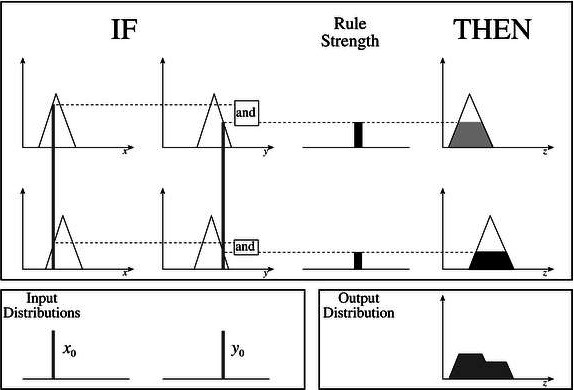
\includegraphics[scale = 0.5]{mamdani_process.jpg}

\section*{Detalles de Implementaci\'on}
Para implementar el sistema es necesario especificar su estructura, d\'igase las reglas que lo conforman,
las variables y sus posibles clasificaciones difusas, as\'i como la distribuci\'on de los valores que puede
tomar dicha variable y su grado de pertenencia al conjunto (funciones de membres\'ia). Para facilitar este trabajo
se define un simple DSL (Domain Specific Language) y un mini-parser para interpretar dichas reglas y convertirlas
a los objetos corrrespondientes de Python $\epsilon$.
\paragraph{}
El DSL implementado sigue la siguiente gram\'atica:

\begin{verbatim}
    Program                   --> SetsDefinitions FuzzySetsConformations Rules

    SetsDefinitions           --> identifier num num num : FuzzySet
    SetsDefinitions           --> identifier num num num : FuzzySet SetsDefinitions

    FuzzySet                  --> identifier
    FuzzySet                  --> identifier , FuzzySet

    FuzzySetsConformations    --> = identifier SetDescription
    FuzzySetsConformations    --> = identifier SetDescription FuzzySetsConformations

    SetDescription            --> function NumList
    NumList                   --> Num NumList
    NumList                   --> EPSILON

    Rules                     --> If Formula Then Statement Rules
    Rules                     --> EPSILON

    Formula                   --> Statement
    Formula                   --> Statement and Formula

    Statement                 --> identifier is identifier
    Statement                 --> not Statement
    Statement                 --> ( Formula )

    identifier = [aA-Zz]+
    num = [0-9]+
    function = TrapezoidSet | TriangularSet
\end{verbatim}
\paragraph{}
Desde un punto de vista program\'atico, cada operacion l\'ogica \textbf{and}, \textbf{not} y \textbf{or} se
representan como \textbf{$min$}, \textbf{$1 - x$} y \textbf{$max$} respectivamente. Para la desfusificaci\'on
se implementan los m\'etodos \textbf{centroide}, \textbf{bisector}, \textbf{promedio de los m\'aximos} y 
\textbf{primer M\'aximo}. Existen la clase \textbf{FuzzyVar} que representa una variable y la clase 
\textbf{FuzzyClassification} que representa un conjunto disfuso sobre alguna variable. Este conjunto
recibe posibles valores de dominio (un m\'inimo, un m\'aximo y un espaciado) y luego, cuando se parsea
la definici\'on de un sistema, el conjunto se transforma en trapezoide o triangular en dependencia de la
funci\'on de membres\'ia que se especifique. Para determinar el mapeo entre valores de dominio e imagen,
se utilizan los arrays de numpy, sobre los cuales es muy c\'omodo luego utilizar las operaciones de multiplicaci\'on,
suma, hallar m\'aximo, m\'inimo y calcular los \'indices de los m\'aximos y m\'inimos.
La clase \textbf{Rule} agrupa una regla, recogiendo los antecedentes y la consecuencia y ofreciendo una interfaz
para calcular el aporte de los antecedentes (metodo Fired y Apply).

\paragraph{}
El engranage principal es la clase abstracta \textbf{FuzzySystem}, que guarda un diccionario de variables
y clasificaciones, y una lista de reglas. La idea es que cada sistema implemente el m\'etodo \textbf{evaluate}.
Las clases concretas MamdaniFuzzySystem implementa la evaluaci\'on de las reglas truncando el domino de 
las consecuencias de las reglas que se disparen (o sea, hallando el m\'inimo entre el dominio de la consecuencia
y la contribuci\'on de los antecedentes que sea mayor que 0).

El siguiente m\'etodo es un claro resumen de lo que pasa en el sistema:

\begin{verbatim}
    def evaluate(self, inputVariables: Dict[str, float]):
        # Search for rules that fires with variables's input
        input_: Dict[FuzzyVar, float] = {
            key: inputVariables[key.name]
            for key in self.sets.keys()
            if key.name in inputVariables
        }
        firedRules = self.evaluate_rules(input_)

        self.aggregate_rules(firedRules)

        self.desfuzzify(firedRules)

        return firedRules
\end{verbatim}

\begin{enumerate}
    \item Se reciben las variables de entrada con los valores que se quieren evaluar.
    \item Se busca en cada regla, una que contenga las variables que se suministran y que la contribuci\'on de sus antecedentes sea mayor que 0.
    \item Se agrupan las reglas utilizando la operaci\'on m\'aximo.
    \item Se desfusifica el resultado (Luego de la agrupaci\'on lo que obtenemos es un conjunto disfuso).
\end{enumerate}

\paragraph{}
Este proceso se ve de manera gr\'afica en la siguiente figura:

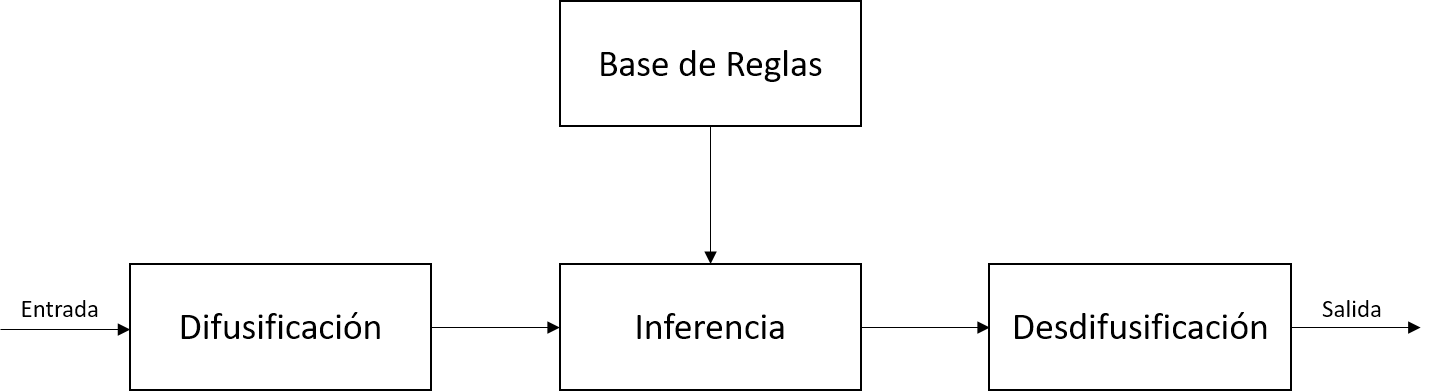
\includegraphics[scale=0.3]{graph.png}

\section*{App}
En el proyecto se provee del m\'odulo \textbf{fis.py} que sirve como driver para cargar un sistema de 
inferencia y suministrarle entradas para obtener los resultados. Veamos las posibles opciones que brinda
esta app y luego resolvamos un problema con ella:

\begin{verbatim}
$ ./fis.py --help
  usage: fis.py [-h] [-l FILE] [-s] [-r INPUT] 
                [-e <VariableName:Value> [<VariableName:Value> ...]]
                [-m {maximum,centroid,mom,bisector}] [-t {mamdani,larsen}]

  Tool for managing Mamdani and Larsen Fuzzy Inference Systems

  optional arguments:
    -h, --help            show this help message and exit
    -l FILE, --load FILE  File containing the FIS definition with the specified grammar.
    -s, --show            Show the Domain Specific Language available for 
                          the construction of FIS.
    -r INPUT, --read-input INPUT
                          Read input variables from a file. This options requires --load.
    -e <VariableName:Value> [<VariableName:Value> ...], 
                            --eval <VariableName:Value> [<VariableName:Value> ...]
                          Provides inputVariables to the loaded system. 
                          Should be used in conjuction with --load.
    -m {maximum,centroid,mom,bisector}, --method {maximum,centroid,mom,bisector}
                          Defuzzification method used by the system. 
                          Defaults to centroid.
    -t {mamdani,larsen}, --type {mamdani,larsen}
                          Define the model to use in the system. 
                          Defaults to mamdani.
\end{verbatim}

\paragraph{}
Consideremos el problema de determinar la velocidad de un fan, tomando como referencia la humedad
y la temperatura. La temperatura la podemos clasisficar como \textit{Cold, Medium y Hot}, la humedad
como \textit{Dry, Normal, Wet} y la velocidad del fan como \textit{Slow, Moderate, Fast}. Queremos saber
si por ejemplo tenemos una humedad de 60 y una temperatura de 18 grados, entonces que velocidad debe
tener el fan?

Modelemos nuestro sistema:

\begin{verbatim}
### FILE: FanSpeedControl.fis

Temperature 10 40 100 : Cold, Medium, Hot
Humidity 20 100 100 : Dry, Normal, Wet
Speed 0 100 100 : Slow, Moderate, Fast

= Cold TriangularSet 10 25 10
= Medium TriangularSet 15 35 25
= Hot TriangularSet 25 40 40

= Dry TriangularSet 60 100 100
= Wet TriangularSet 20 60 20
= Normal TrapezoidSet 30 50 70 90

= Slow TriangularSet 0 50 0
= Moderate TriangularSet 10 90 50
= Fast TriangularSet 50 100 100

if Temperature is Cold and Humidity is Wet then Speed is Slow
if Temperature is Cold and Humidity is Normal then Speed is Slow
if Temperature is Medium and Humidity is Wet then Speed is Slow
if Temperature is Medium and Humidity is Normal then Speed is Moderate
if Temperature is Cold and Humidity is Dry then Speed is Moderate
if Temperature is Hot and Humidity is Wet then Speed is Moderate
if Temperature is Hot and Humidity is Normal then Speed is Fast
if Temperature is Hot and Humidity is Dry then Speed is Fast
if Temperature is Medium and Humidity is Dry then Speed is Fast
\end{verbatim}

Carguemos el sistema en nuestra app y veamos que devuelve:

\begin{verbatim}
$ ./fis.py --load systems/FanSpeedControl.fis -e Temperature:18 Humidity:60
  {Speed: 37.14222809335096}
\end{verbatim}

Usemos otro m\'etodo de desfusificaci\'on:
\begin{verbatim}
$ ./fis.py --load systems/FanSpeedControl.fis -e Temperature:18 Humidity:60 -m bisector
  {Speed: 33.333333333333336}
\end{verbatim}

Y usando Larsen ?

\begin{verbatim}
$ ./fis.py --load systems/FanSpeedControl.fis -e Temperature:18 Humidity:60 -t larsen
  {Speed: 33.45878031356237}
\end{verbatim}

\paragraph{}
Como podemos ver el sistema es capaz de adoptar una velocidad moderada para una temperatura
media y una humedad normal, tanto con Larsen, como con Mamdani, adem\'as, se puede apreciar la
diferencia entre la desusificaci\'on usando centroide y usando bisector, aunque ambos m\'etodos, al
ser puntos de equilibrio, obtienen resultados relativamente parecidos. En general, para este problema,
encontramos que el modelo de Mamdani es m\'as adecuado a lo esperado del sistema. 
\end{document}
